\documentclass[fleqn]{article}
\oddsidemargin 0.0in
\textwidth 6.0in
\thispagestyle{empty}
\usepackage{import}
\usepackage{amsmath}
\usepackage{mathtools}
\usepackage{graphicx}
\usepackage{flexisym}
\usepackage{calligra}
\usepackage{amssymb}
\usepackage{bigints} 
\usepackage[english]{babel}
\usepackage[utf8x]{inputenc}
\usepackage{float}
\usepackage[colorinlistoftodos]{todonotes}


\DeclareMathAlphabet{\mathcalligra}{T1}{calligra}{m}{n}
\DeclareFontShape{T1}{calligra}{m}{n}{<->s*[2.2]callig15}{}
\newcommand{\scriptr}{\mathcalligra{r}\,}
\newcommand{\boldscriptr}{\pmb{\mathcalligra{r}}\,}

\definecolor{hwColor}{HTML}{442020}

\begin{document}

  \begin{titlepage}

    \newcommand{\HRule}{\rule{\linewidth}{0.5mm}}

    \center

    \begin{center}
      
\includegraphics[height=11cm, width=11cm]{asu.png}
    \end{center}

    \vline

    \textsc{\LARGE Classical Parts/Field/Matter III}\\[1.5cm]

    \HRule \\[0.5cm]
    { \huge \bfseries Homework Four}\\[0.4cm] 
    \HRule \\[1.0cm]

    \textbf{Behnam Amiri}

    \bigbreak

    \textbf{Prof: Samuel Teitelbaum}

    \bigbreak

    \textbf{{\large \today}\\[2cm]}

    \vfill

  \end{titlepage}

  \begin{enumerate}
    \item \textbf{9.18 (30 points)} The index of refraction of diamond is $2.42$. Construct the graph analogous to Fig. $9.16$ for the air/diamond 
    interface. (Assume  $\mu_1=\mu_2=\mu_0$.) In particular, calculate (a) the amplitudes at normal incidence, (b) Brewster’s angle, and (c)
    the “crossover” angle, at which the reflected and transmitted amplitudes are equal.

      \begin{figure}[h!]
        \centering
        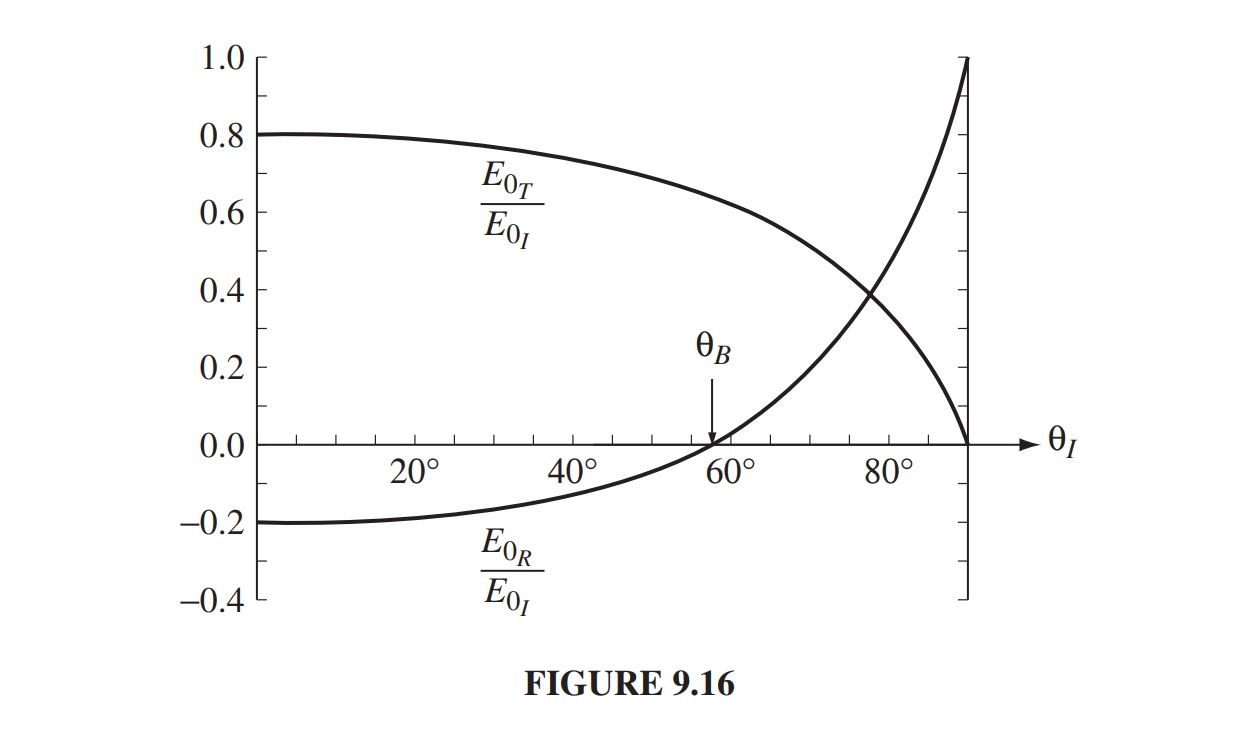
\includegraphics[height=6cm, width=10cm]{figure9.16.JPG}
      \end{figure}

      \textcolor{hwColor}{
        \\
        We are given the index of refraction which is $2.42$ and we are assuming $\mu_1=\mu_2=\mu_0$. So we have:
        \\
        \\
        $
          \beta=\dfrac{\mu_1 ~ v_1}{\mu_2 ~ v_2}=\dfrac{\mu_1 ~ n_2}{\mu_2 ~ n_1}
          =\dfrac{\mu_0 ~ n_2}{\mu_0 ~ n_1}=\dfrac{n_1}{n_2}=\dfrac{2.42}{1}
          \\
          \\
          \\
          \therefore ~~~ \boxed{
            \dfrac{n_2}{n_1}=2.42=\beta
          } ~~~~ \checkmark
          \\
          \\
          \rule{15cm}{1pt}
          \\
          \\
        $
        \textbf{(a)}
        \\
        \\
        $
          \tilde{{E_0}_R}=\left(\dfrac{\alpha-\beta}{\alpha+\beta}\right) \tilde{{E_0}_I}
        $
        \\
        \\
        So we have to find the value of $\alpha$:
        \\
        \\
        $
          \alpha=\dfrac{\sqrt{1-\left[\dfrac{n_1}{n_2} sin(\theta_I)\right]^2}}{cos(\theta_I)}
          =\dfrac{\sqrt{1-\left[2.42 sin(0)\right]^2}}{cos(0)}
          \\
          \\
          \\
          \therefore ~~~ \boxed{
            \alpha=1
          } ~~~~ \checkmark
          \\
          \\
          \tilde{{E_0}}_R=\left(\dfrac{\alpha-\beta}{\alpha+\beta}\right) \tilde{{E_0}}_I
          \Longrightarrow \dfrac{\tilde{{E_0}}_R}{\tilde{{E_0}}_I}=\left(\dfrac{\alpha-\beta}{\alpha+\beta}\right)
          =\dfrac{1-2.42}{1+2.42}
          \\
          \\
          \\
          \therefore ~~~ \boxed{
            \dfrac{\tilde{{E_0}}_R}{\tilde{{E_0}}_I}=−0.4152
          } ~~~~ \checkmark
          \\
          \\
          \\
          \therefore ~~~ \boxed{
            \dfrac{\tilde{{E_0}}_T}{\tilde{{E_0}}_I}=\dfrac{2}{\alpha+\beta}
            =\dfrac{2}{1+2.42}
            =0.5847
          } ~~~~ \checkmark
          \\
          \\
          \rule{15cm}{1pt}
          \\
          \\
          \textbf{(b)}
          \\
          \\
          tan(\theta_B) \approx \dfrac{n_2}{n_1} \Longrightarrow \theta_B=Arctan(\dfrac{n_2}{n_1})
          =Arctan(2.42)
          \\
          \\
          \\
          \therefore ~~~ \boxed{
            \theta_B=67.5484^{\circ}
          } ~~~~ \checkmark
          \\
          \\
          \rule{15cm}{1pt}
          \\
          \\
          \textbf{(c)}
          \\
          \\
        $
        We are asked to find the angle when the reflected and transmitted amplitudes are equal, therefore:
        \\
        \\
        $
          \tilde{{E_0}}_T=\tilde{{E_0}}_R \Longrightarrow \left(\dfrac{2}{\alpha+\beta}\right) \tilde{{E_0}}_I
          =\left(\dfrac{\alpha-\beta}{\alpha+\beta}\right)\tilde{{E_0}}_I
          \\
          \\
          \Longrightarrow \left(\dfrac{2}{\alpha+\beta}\right)=\left(\dfrac{\alpha-\beta}{\alpha+\beta}\right)
          \\
          \\
          \\
          \therefore ~~~ \boxed{
            2=\alpha-\beta ~~ \text{or} ~~ \alpha=2+\beta
          } ~~~~ \checkmark
          \\
          \\
          \\
          \alpha=\dfrac{\sqrt{1-\left[\dfrac{n_1}{n_2} sin(\theta_I)\right]^2}}{cos(\theta_I)}
          \Longrightarrow 2+\beta=\dfrac{\sqrt{1-\left[2.42 \times sin(\theta_I)\right]^2}}{cos(\theta_I)}
          \\
          \\
          \\
          \left(2+\beta\right)^2=\dfrac{1- \dfrac{1}{\beta^2} ~ sin^2(\theta_I)}{cos^2(\theta_I)} 
          \Longrightarrow \left(2+\beta\right)^2 cos^2(\theta_I)=1-\dfrac{sin^2(\theta_I)}{\beta^2} 
          \\
          \\
          \left(2+\beta\right)^2 \left(1-sin^2(\theta_I)\right)-1+\dfrac{sin^2(\theta_I)}{\beta^2}=0
          \Longrightarrow \dfrac{\left(2+\beta\right)^2-1}{\left(2+\beta\right)^2-\dfrac{1}{\beta^2}}=sin^2(\theta_I)
          \\
          \\
          \\
          \Longrightarrow sin(\theta_I)=\sqrt{\dfrac{\left(2+\beta\right)^2-1}{\left(2+\beta\right)^2-\dfrac{1}{\beta^2}}}
          \Longrightarrow
          \theta_I=Arcsin \left[
            \sqrt{\dfrac{\left(2+\beta\right)^2-1}{\left(2+\beta\right)^2-\dfrac{1}{\beta^2}}}
          \right]
          \\
          \\
          \\
          \therefore ~~~ \boxed{
            \theta_I=78.0574^{\circ}
          } ~~~~ \checkmark
          \\
          \\
        $
      }

      \begin{figure}[h!]
        \centering
        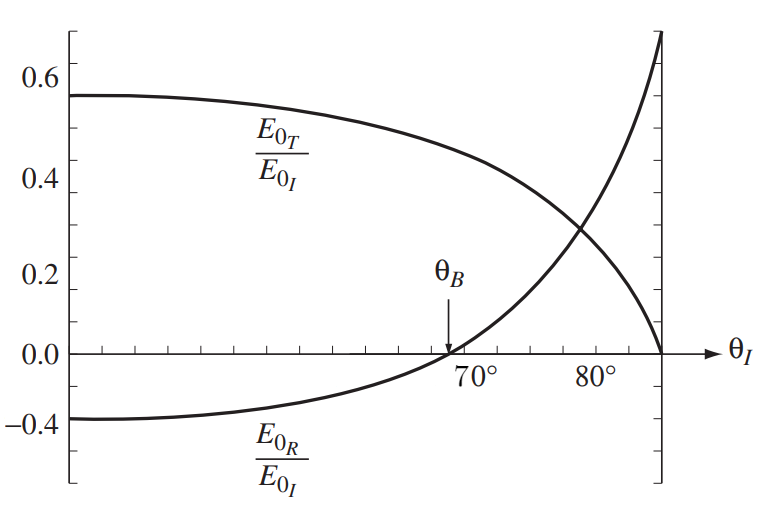
\includegraphics[height=6cm, width=10cm]{YY.png}
      \end{figure}

    \pagebreak

    \item \textbf{9.39 (70 points)} According to Snell’s law, when light passes from an optically dense medium into a less dense one ($n_1 > n_2$) the 
    propagation vector \textbf{k} bends away from the normal (Fig. 9.28). In particular, if the light is incident at the \textbf{critical angle}
    $$
      \theta_c \equiv sin^{-1} \left(n_2/n_1\right)
    $$
    then $\theta_T=90^{\circ}$,  and the transmitted ray just grazes the surface. If $\theta_I$ exceeds $\theta_c$,there is no refracted ray at all, only a 
    reflected one (this is the phenomenon of \textbf{total internal reflection}, on which light pipes and fiber optics are based). But the fields are 
    not zero in medium $2$; what we get is a so-called \textbf{evanescent wave}, which is rapidly attenuated and transports no energy into medium $2$.
    \\
    \emph{6 The evanescent fields can be detected by placing a second interface a short distance to the right of
    the first; in a close analog to quantum mechanical tunneling, the wave crosses the gap and reassembles
    to the right. See F. Albiol, S. Navas, and M. V. Andres, Am. J. Phys. 61, 165 (1993).}

    \begin{figure}[h!]
      \centering
      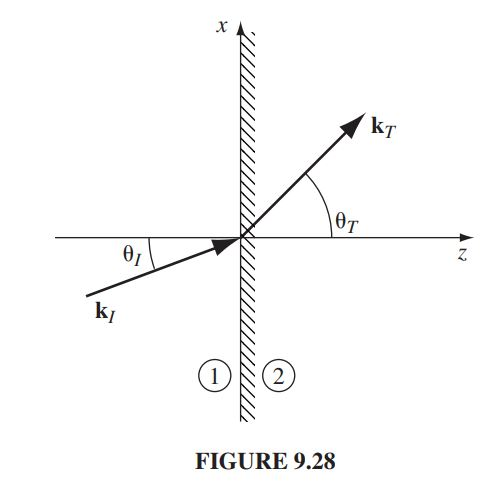
\includegraphics[height=8cm, width=8cm]{figure9.28.JPG}
    \end{figure}

    A quick way to construct the evanescent wave is simply to quote the results of Sect. 9.3.3, with $k_T=\omega ~ n_2/c$ and
    $$
    \mathbf{K}_T=k_T \left(sin ~ \theta_T ~ \hat{x}+cos ~ \theta_T ~ \hat{z}\right)
    $$
    the only change is that 
    $$
      sin ~ \theta_T=\dfrac{n_1}{n_2} ~ sin ~ \theta_I
    $$
    is now greater than $1$, and 
    $$
      cos ~ \theta_T=\sqrt{1-sin^2 ~ \theta_T}=i ~ \sqrt{sin^2 ~ \theta_T-1}
    $$
    is imaginary. (Obviously, $\theta_T$ can no longer be interpreted as an \emph{angle}!)

    \begin{enumerate}
      \item Show that
      $$
        \mathbf{\tilde{E}}_T(\mathbf{r}, t)=\mathbf{\tilde{E_0}}_T ~ e^{-\kappa z} ~ e^{i(kx-\omega ~ t)},
      $$
      where 
      $$
        \kappa \equiv \dfrac{\omega}{c} \sqrt{\left(n_1 ~ sin ~ \theta_I\right)^2-n_2^2} ~~~~~ \text{and} ~~~~~ k \equiv \dfrac{\omega ~ n_1}{c} sin ~ \theta_I 
      $$
      This is a wave propagating in the $x$ direction (\emph{parallel} to the interface!), and attenuated in the $z$ direction.

        % \textcolor{hwColor}{
        %   \\
        % }

      \item Noting that $\alpha$ (Eq. 9.108) is now imaginary, use Eq. $9.109$ to calculate the reflection coefficient for polarization 
      parallel to the plane of incidence. [Notice that you get $100\%$ reflection, which is better than at a conducting 
      surface (see,for example, Prob. 9.22).]

        % \textcolor{hwColor}{
        %   \\
        % }

      \item Do the same for polarization perpendicular to the plane of incidence (use the
      results of Prob. 9.17).

        % \textcolor{hwColor}{
        %   \\
        % }

      \item In the case of polarization perpendicular to the plane of incidence, show that
      the (real) evanescent fields are
      $$
        \begin{rcases*}
          \mathbf{E(r},t)=E_0 ~ e^{-\kappa z} ~ cos(kx-\omega ~ t) ~ \mathbf{\hat{y}},
          \\
          \mathbf{B(r},t)=\dfrac{E_0}{\omega} ~ e^{-\kappa z} \left[
            \kappa ~ sin(kx-\omega t) ~ \mathbf{\hat{x}}+k ~ cos(kx-\omega t) \mathbf{\hat{z}}.
          \right]
        \end{rcases*}
      $$

        % \textcolor{hwColor}{
        %   \\
        % }

      \item Check that the fields in (d) satisfy all of Maxwell’s equations (Eq. $9.67$).
      
        % \textcolor{hwColor}{
        %   \\
        % }


      \item For the fields in (d), construct the Poynting vector, and show that, on average, no energy is transmitted in the z direction.
      
        % \textcolor{hwColor}{
        %   \\
        % }

    \end{enumerate}

  \end{enumerate}

\end{document}
